\chapter{Multiscale Score Matching}
\label{ch:msma}

In this chapter, I will outline the main idea behind Multiscale Score Matching Analysis (MSMA); my method for outlier detection via score norms. In this work, we made use of Noise Conditioned Score Network (NCSN)~\cite{Song2019}, which have now been superseded by diffusion models. However, this laid the foundation and proof of concept on which the rest of my research was developed.

\section{Multiscale Score Analysis}

Consider taking the L2-norm of the score function:
$ \norm{ s(x) } = \norm{ \nabla_{x} \log p(x)  } = \norm{ \frac{\nabla_{x}\text{~}p(x)}{p(x)} } $.
One can ask the question: Is the norm of a score function sufficient to identify samples with low density $p(x)$?

Since the data density term appears in the denominator, a high likelihood will correspond to a low norm. In contrast, out-of-distribution samples should have a low likelihood with respect to the in-distribution log density (i.e. $p(x)$ is small), and we can expect them to have high score norms. However, if these outlier points reside in ``flat" regions with very small gradients (or perhaps in a local mode),  their score norms can be low despite the point belonging to a low density region. 
\figref{fig:toy_gmm} illustrates a possible scenario of outlying points.
This is our first indicator informing us that a true score norm may not be sufficient for detecting outliers. 

I empirically validate this intuition by considering score estimates for a relatively simple toy dataset: FashionMNIST. Following the denoising score matching objective in \eqnref{eq:ncsn_dsm}, one can obtain multiple estimates of the true score by using different noise distributions $q_{\sigma}(\tilde{x}|x)$. Like \cite{Song2019}, I choose the noise distributions to be a zero-centered Gaussian scaled according to $\sigma_i$. Recall that the scores for samples perturbed by the lowest $\sigma$ noise should be closest to the true score. My analysis shows that this alone was inadequate at separating inliers from OOD samples.

\begin{figure}[tbhp]
\small
\label{fig:scores}
\centering
\begin{subfigure}[b]{\textwidth}
    \centering
    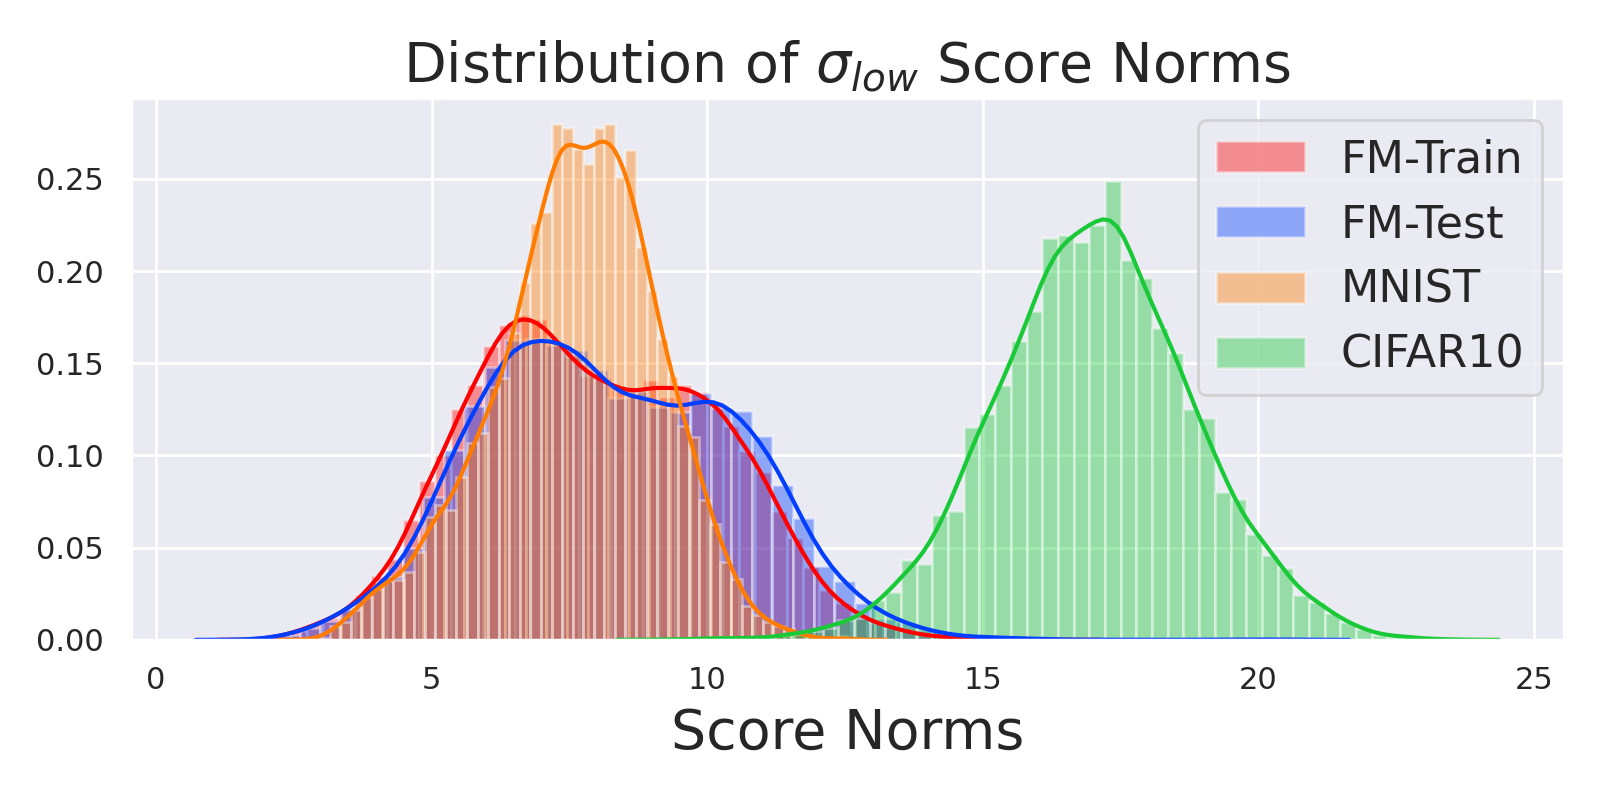
\includegraphics[width=0.9\textwidth]{figures/low_sigma_FvM_tight.png}
    \caption{1D score estimates from a model trained on FashionMNIST (FM)}
    \label{fig:score_norms}
\end{subfigure}
\hfill
\begin{subfigure}[b]{\textwidth}
    \centering
    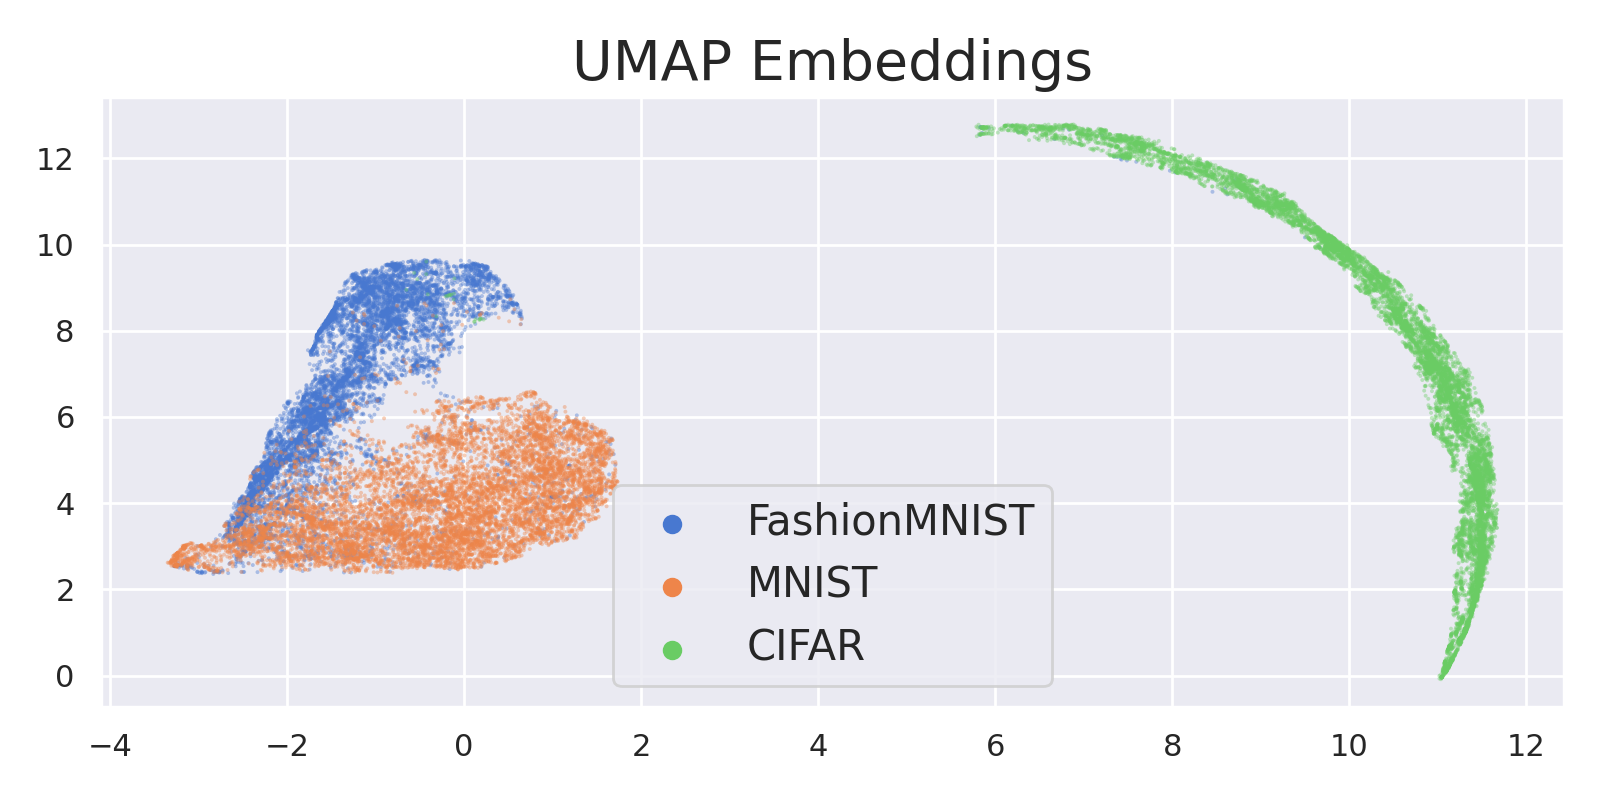
\includegraphics[width=0.9\textwidth]{figures/umap_fashion_tight.png}
    \caption{UMAP visualization of 10-dimensional score estimates from a model trained on FashionMNIST}
    \label{fig:umap}
\end{subfigure}

\caption{Visualizing the need for a multiscale analysis. In (a), I plot the scores corresponding to the lowest sigma estimate. In (b), I plot the UMAP embedding of the $L=10$ dimensional vectors of score norms. Here we see a better separation between FashionMNIST and MNIST when using estimates from \textit{multiple} scales rather than the one that corresponds to the true score only.}
\end{figure}


\subsection{Scales and Neighborhoods}
\label{neighborhoods}

\begin{figure}[tbhp]
\label{fig:toy_gmm}
\centering
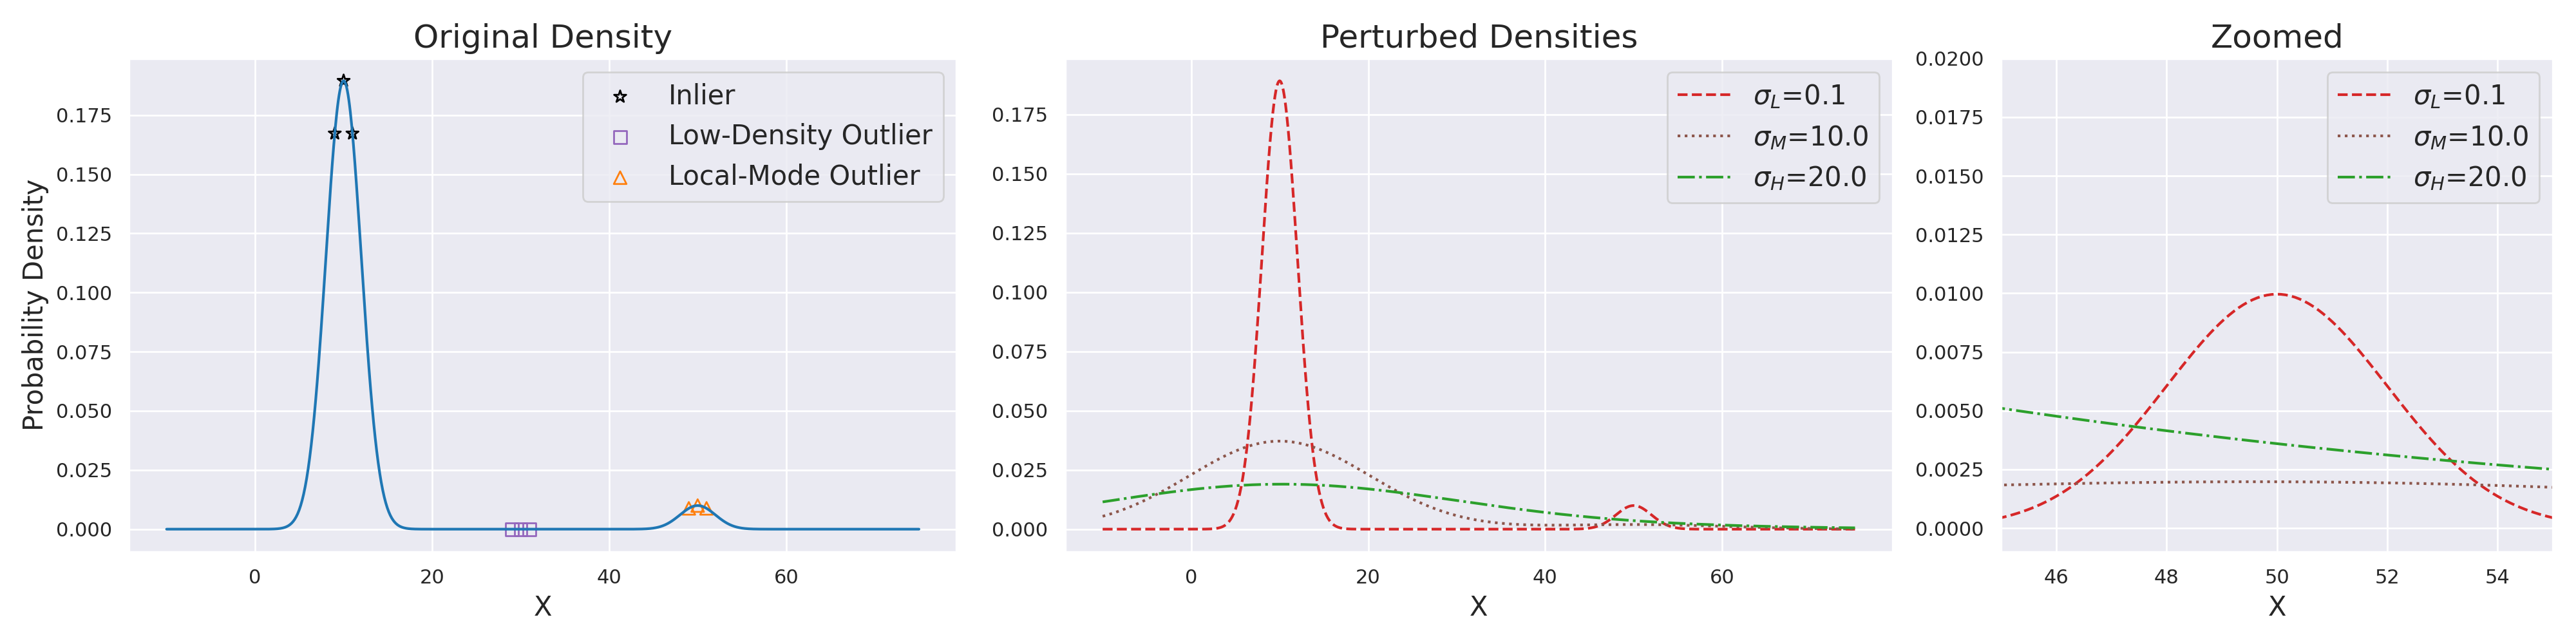
\includegraphics[width=\linewidth]{figures/gmm_plot_tight.png}
\caption{A toy GMM to visualize my analysis with the three regions of interest I will be exploring. Further, I show the Gaussian perturbed versions of the original distribution with (L)ow, (M)edium, and (H)igh noise levels, along with a plot zoomed into the local-mode outliers. Note the effect of different scales on this region: only the largest scale results in a gradient in the direction of the inliers.}
\end{figure}

To my knowledge multiscale score analysis has not been explored in the context of OOD detection. In this section, I present an analysis in order to give an intuition for why multiple scales can be beneficial. Consider the toy distribution shown in \figref{fig:toy_gmm}. We have three regions of interest: an inlier region with high density centered around $x=10$, an outlier region with low density around $x=30$, and a second outlier region with a local mode centered around $x=50$. I will be adding noise of increasing scales to this distribution and observing the resulting score norms.

To begin, recall that sum of two probability distributions is equivalent to a convolution of their probability density functions, as per the law of total probability~\cite{sumisconv}. Thus, I can analytically compute the perturbed distribution, as I know the parameters for both the base distribution (a Gaussian Mixture Model) and the noise distribution $\mathcal{N}(0; \sigma)$. This not only allows us to visualize perturbations of our toy distribution, but also analytically compute the score estimates given any $\sigma_i$.

On the left hand side, we have the initial density with no perturbation. Note how points within the low-density region and at the peak of the local-mode will have small gradients due to being inside a flat area. As we perturb the samples, we smooth the original density, causing it to widen. The relative change in density at each point is dependent on neighboring modes. A large scale perturbation will proportionally take a larger neighborhood into account at each point of the convolution. Therefore, at a sufficiently large scale, nearby outlier points gain context from in-distribution modes. This results in an increased gradient signal in the direction of inliers. 

\begin{figure}[tbhp]

\centering
\begin{subfigure}[b]{0.45\textwidth}
    \centering
    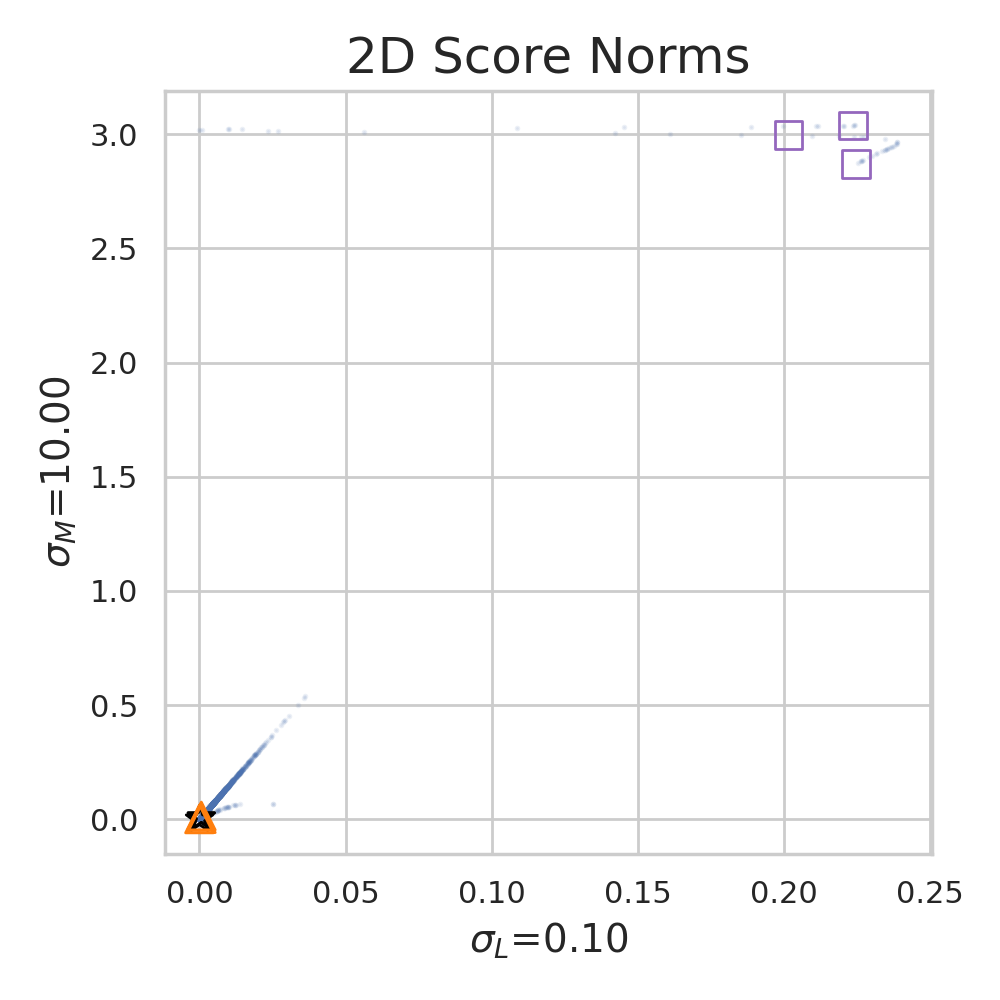
\includegraphics[scale=0.3]{figures/scatter_2d_white.png}
    % \caption{}
    \label{fig:score_norms_2d}
\end{subfigure}
% \hfill
\begin{subfigure}[b]{0.45\textwidth}
    \centering
    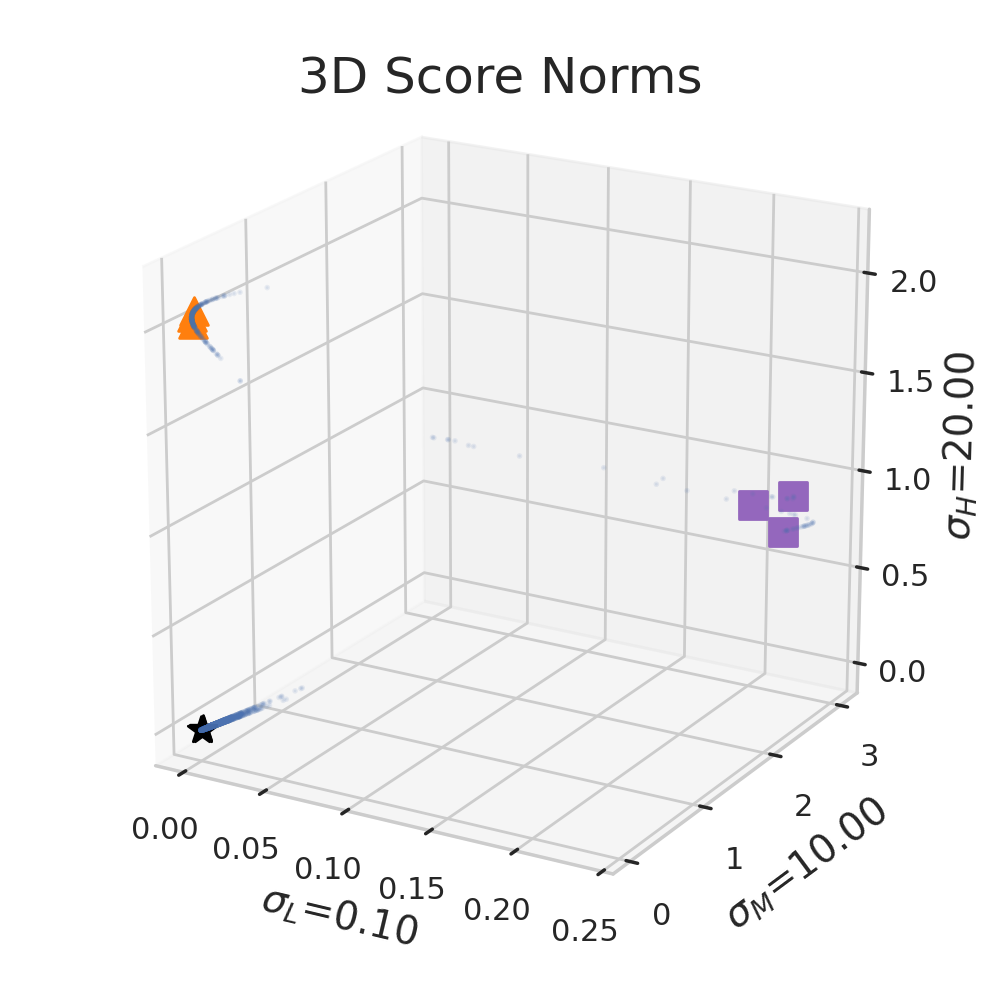
\includegraphics[scale=0.3]{figures/scatter_3d_white.png}
    % \caption{}
    \label{fig:score_norms_3d}
\end{subfigure}
\caption{In (a) observe that Low-Density outliers have comparatively high gradient norms for both $\sigma_{L}$ and $\sigma_{M}$. However at this scale, Local-Mode points still have very small norms, causing them to be tightly packed around the in-distribution points. In (b) we see that Local-Mode outliers achieve a gradient signal only when a sufficiently high scale is used, $\sigma_{H}=20$.}
\label{fig:norm_plots}
\end{figure}

Figure~\ref{fig:norm_plots} plots the score norms of samples generated from the original density along with markers indicating our key regions. Note how even a small scale perturbation ($\sigma_{L}=0.1$) is enough to bias the tails of the density towards the outliers. However, a medium scale ($\sigma_{M}=10$) Gaussian perturbation is still not wide enough to reach the inlier region from the Local-Mode outlier densities, causing them to simply smooth away into flat nothingness. It is only after we perform a large scale ($\sigma_{H}=20$) perturbation that the in-distribution mode gets taken into account, resulting in a higher gradient norm. Note that the flat Low-Density outliers will not see the same increase in gradients. This analysis allows one to intuit that larger noise levels account for a larger neighborhood context. We surmise that given a sufficiently large scale, we can capture gradient signals from distant outliers.

Figure~\ref{fig:norm_plots} plots the score norms of samples generated from the original density along with markers indicating our key regions. Note how even a small scale perturbation ($\sigma_{L}=0.1$) is enough to bias the density of the Low-Density outliers towards the nearby in-distribution mode. A medium scale ($\sigma_{M}=10$) Gaussian perturbation is still not wide enough to reach the inlier region from the Local-Mode outlier densities, causing them to simply smooth away into flat nothingness. It is only after we perform a large scale ($\sigma_{H}=20$) perturbation that the in-distribution mode gets taken into account, resulting in a higher gradient norm.
% Note that the flat Low-Density outliers will not see the same increase in gradients. This illustrates the notion that no one scale is appropriate to detect all outliers.
This analysis allows us to intuit that larger noise levels account for a larger neighborhood context. We surmise that given a sufficiently large scale, we can capture gradient signals from distant outliers.

However, it is imperative to note that no single scale is guaranteed to work for \textit{all} outliers. Consider outliers close to inlier modes such as the samples between Low-Density outliers and Inliers in \figref{fig:toy_gmm}. $\sigma_H$ results in an overlap in the score distribution of inliers and Low-Density outliers. This makes it difficult to differentiate the aforementioned ``in-between" outliers from the in-distribution samples. However, this large scale was necessary to get a big enough neighborhood context in order to capture the more distant Local-Mode outliers. Therefore, I postulate that a \emph{range} of scales is necessary for separating outliers.

Admittedly, selecting this range according to the dataset is not a trivial problem. In \tempcite{song2020improved} outlined some techniques for selecting $\{\sigma_i\}_{i=1}^L$ for NCSNs from the perspective of generative modelling. Perhaps there is a similar analog to OOD detection. I did not perform such a statistical analysis for this work and used the default range for NCSN in all my experiments. 

However, we observed that my defaults are surprisingly generalizable, evident by the fact that all my experiments in Section~\ref{experiments} were performed with the same scale range. In Section~\ref{hyperparams}, we further analyze how varying the scale range effects downstream accuracy and observe that our defaults already provide near optimal performance.

\section{Experiments}
\label{experiments}

\subsection{Hyperparameter Analysis}
% \cbstart
\label{hyperparams}